\documentclass[10pt]{article}
\usepackage[polish]{babel}
\usepackage[utf8]{inputenc}
\usepackage[T1]{fontenc}
\usepackage{graphicx}
\usepackage[export]{adjustbox}
\graphicspath{ {./images/} }
\usepackage{amsmath}
\usepackage{amsfonts}
\usepackage{amssymb}
\usepackage[version=4]{mhchem}
\usepackage{stmaryrd}

\title{LIGA MATEMATYCZNA \\
 im. Zdzisława Matuskiego \\
 LISTOPAD 2013 \\
 SZKOŁA PODSTAWOWA }

\author{}
\date{}


\begin{document}
\maketitle
\section*{ZADANIE 1.}
Oblicz sumę liczb w pustych polach diagramu, jeżeli liczba w każdym polu w rzędzie wyższym jest sumą dwóch liczb z niższego rzędu sąsiadujących z nim.\\
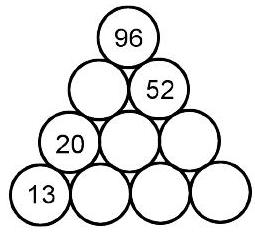
\includegraphics[max width=\textwidth, center]{2024_11_21_6d866016f49aaf506f81g-1}

\section*{ZADANIE 2.}
Pięciu chłopców ważyło się parami każdy z każdym. Otrzymano następujące rezultaty: 90 kg , \(92 \mathrm{~kg}, 93 \mathrm{~kg}, 94 \mathrm{~kg}, 95 \mathrm{~kg}, 96 \mathrm{~kg}, 97 \mathrm{~kg}, 98 \mathrm{~kg}, 100 \mathrm{~kg}, 101 \mathrm{~kg}\). Podaj łączną wagę tych chłopców.

\section*{ZADANIE 3.}
Obwód prostokąta zbudowanego z dwudziestu jednakowych kwadratów jest równy 126. Oblicz pole prostokąta. Rozważ wszystkie możliwości.

\section*{ZADANIE 4.}
Ogrodnik włożył 80 gruszek do 12 koszyków w taki sposób, że w każdym koszyku znalazła się co najmniej jedna gruszka. Czy jest możliwe, że w każdym koszyku znajduje się inna liczba gruszek?

\section*{ZADANIE 5.}
W upalny dzień w kawiarni usiedli Ania, Antek, Bartek, Czarek i Darek. Wszyscy zamówili zimne napoje i każdy zamówił coś innego. Ustal kto zamówił jaki napój, jeżeli

\begin{itemize}
  \item Antek jako jedyny lubi oranżadę;
  \item Bartek nie lubi napojów gazowanych;
  \item Czarek nie lubi coca-coli ani wody gazowanej;
  \item Ania pije tylko wodę gazowaną;
  \item zamówiono też fantę i wodę niegazowaną.
\end{itemize}

\end{document}